\chapter{Google PageRank}
% El PageRank, nombrado en honor a Larry Page, es una de las medidas de centralidad de los nodos de un grafo más conocidas. Ésta es utilizada para ordenar los sitios web en los resultados de búsqueda de Google, de acuerdo a su importancia.

El algoritmo de PageRank fue desarrollado en 1996 en la Universidad de Stanford por Larry Page y Sergey Brin, los cuales fueron los fundadores de Google.

Este algoritmo se basa en la idea de que sitios web importantes tienen muchos vínculos que apuntan hacia ellos, lo que conduce a pensar en la web como una red ponderada orientada.

Existen muchos otros algoritmos, algunos más eficientes, pero la importancia de PageRank se sustenta en el poder económico de Google.

Ilustraremos el algoritmo de PageRank con un ejemplo sencillo:

Ejemplo:

Consideremos 5 páginas web distintas a las que denotaremos por 1, 2, 3, 4, y 5, y cuyo grafo es:
\vspace{3cm}

Pasos:
\begin{enumerate}
\item Determinar la matriz de adyacencia. Algunos autores denotan la matriz de de adyacencia por M en el protocolo de PageRank

\[
M = \begin{pmatrix}
0 & 0 & 1 & 1 & 1 \\
0 & 0 & 0 & 0 & 1 \\
1 & 0 & 0 & 1 & 1 \\
1 & 0 & 1 & 0 & 0 \\
1 & 1 & 0 & 0 & 0
\end{pmatrix}
\]

\item Sumamos los elementos de cada una de las columnas.

\[
\begin{matrix}
3 & 1 & 2 & 2 & 3
\end{matrix}
\]

Estas sumas representan el número de links que salen del nodo o vértice de la página $p_j$, es decir: 

$I(p_j) \equiv \text{Importancia de la página j}$

$\mathrm{outdeg}(p_j) \equiv \text{número de links que salen de la página } p_j$

$I(p_i) \equiv \sum\limits_{j \in B_i} \frac{I(p_j}{\mathrm{outdeg}(p_j)}$

$B_i \equiv \text{conjunto de páginas qeu son linkeadas}$

\item Dividimos cada elemento de M por la suma de los elementos de la columna a la cual corresponde y llamaremos a la nueva matriz obtenida $M^\prime$

\[
M^\prime = \begin{pmatrix}
0 & 0 & 1/2 & 1/2 & 1/3 \\
0 & 0 & 0 & 0 & 1/3 \\
1/3 & 0 & 0 & 1/2 & 1/3 \\
1/3 & 0 & 1/2 & 0 & 0 \\
1/3 & 1 & 0 & 0 & 0
\end{pmatrix}
\]

\item El siguiente paso es encontrar un vector $\vec{v}$ (algunos autores lo llaman $\vec{I}$) que represente el PageRank de cada una de las páginas. Como tenemos 5 páginas web le asignamos a $\vec{v}$ como valores $\vec{v} = (a,b,c,d,e)^T$, obteniendo así un vector de dimensión $d=5$.

\item Obtenemos los valores de $\{v_i\}$ a partir de los autovalores de $M^\prime$, tal que:

\[
M^\prime \vec{v} = \lambda \vec{v} \text{ con }\lambda \in R
\]

\item Determinamos los autovalores de $M^\prime$

\[
\lambda_1 = 1; \quad \lambda_2 = \frac{-2}{3}; \quad \lambda_3 = \frac{-1}{2}; \quad \lambda_4 = \frac{-1}{3}; \quad \lambda_5 = \frac{1}{3}
\]

Tomaremos sólo $\lambda = 1$ $\rightarrow M^\prime \vec{v} = \vec{v}$ (Ecuación autoconsistente)

\item Hallamos el autovector asociado a $\lambda = 1$. Obteniendo:

\[
a = 6; \quad b = 1; \quad c = \frac{16}{3}; \quad d = \frac{14}{3}; \quad e = 3
\]

\item Finalmente, Google ordena de mayor a menor las componentes de $\vec{v}$, quedándonos:

\[
\begin{matrix}
& & - & a \\
& & - & c \\
\text{Pantalla} & \rightarrow & - & d \\
& & - & e \\
& & - & b
\end{matrix}
\]
\end{enumerate}

La idea de PageRank de Google es que la importancia de una página viene dada por la cantidad de páginas que se enlazan con ella.

Surgen varios problemas:

\begin{enumerate}
  \item Las matrices hyperlink (hiperenlace) pueden tener billones de entradas en filas y columnas.
  \item Calcular los autovectores es un absurdo computacional.
  \item Los estudios muestran que un nodo (página web) tiene un promedio de 10 enlaces, y las demás entradas de la matriz son cero.
  \item No se encuentra $\lambda = 1$ en la mayoría de los casos.
\end{enumerate}

Por esta razón, un remedio (Patching) del algoritmo de PageRank fue el método de las potencias, en el cual la matriz hiperenlace

\[
H_{ij} \equiv \begin{cases}
\frac{1}{\mathrm{outdeg}(P_j)} & \text{si } P_j \in B_i \\
0 & \text{en otro caso}
\end{cases}
\]

debería converger a una solución autoconsistente

\[
I^{k+1} = H I^k
\]

donde se toma un vector $I^{0}$ y se hace interactuar unas 100 veces y el orden mostrado de las páginas es el de $I^{100}$, ordenadas de mayor a menor. Si se normalizan las columnas de la matriz hipervínculo (hiperenlace) $H$, obtenemos otra matriz hiperenlace normalizada E.

\textbf{La matriz E:} se sabe de la teoría de matrices estocásticas que 1 es uno de sus autovalores. Además, también se sabe que la convergencia de $I^k = E I^{k-1}$ a $I = E I$ depende del segundo autovalor de $\lambda_2$ de E y es un hecho que $I^k = E I^{k-1}$ converge rápidamente si $\abs{\lambda_2}$ es
cercano a cero.

\section{El algoritmo de remiendo (parcheo) general}

Asumamos que el caminante recorre el grafo siguiendo la web con una matriz estocástica E con probabilidad $\alpha$, y con probabilidad $1-\alpha$ podrá ir a cualquier página al azar que sea de su interés. La matriz web de este proceso será:

\[
G \equiv \alpha E + \frac{1-\alpha}{N} \mathds{I} \text{Matriz de Google}
\]

$\mathds{I}$ es una matriz en la cual todas las entradas están establecidas en 1, y N el número de nodos.

Propiedades de G:
\begin{enumerate}
\item Es estocástica
\item Irreducible
\item Primitiva
\item El resultado de determinar el estado auto-consistente no depende del vector Google inicial $I^0$
\end{enumerate}

\begin{figure}[H]
\begin{center}
\begin{tabular}{c c c}
 \begin{tikzpicture}[->,>=stealth',shorten >=1pt,thick]
\tikzset{VertexStyle/.style = {draw,circle,thick,
                               minimum size=0.5cm,
                               font=\bfseries},thick} 
\Vertex[a = 90, d = 2.75]{1}  \Vertex[a = 162, d = 2.75]{2}
\Vertex[a = 234, d = 2.75]{3} \Vertex[a = 306, d = 2.75]{4}
\Vertex[a = 18, d = 2.75]{5}
\Edge[label=$1$](2)(1)
\Edge[label=$1$](1)(5)
\Edge[label=$\frac{1}{2}$](3)(1)
\Edge[label=$\frac{1}{2}$](3)(4)
\Edge[label=$1$](4)(5)
\tikzset{EdgeStyle/.style = {->, bend left}}
\Edge[label=$1$](1)(3)
\end{tikzpicture} 
& \begin{tikzpicture}[->,>=stealth',shorten >=1pt,thick]
\tikzset{VertexStyle/.style = {draw,circle,thick,
                               minimum size=0.5cm,
                               font=\bfseries},thick} 
\Vertex[a = 90, d = 2.75]{1}  \Vertex[a = 162, d = 2.75]{2}
\Vertex[a = 234, d = 2.75]{3} \Vertex[a = 306, d = 2.75]{4}
\Vertex[a = 18, d = 2.75]{5}
\Edge[label=$\frac{1}{10}$](5)(4)
\Edge[label=$\frac{1}{10}$](4)(3)
\Edge[label=$\frac{1}{10}$](3)(2)
\Edge[label=$\frac{3}{5}$](2)(1)
\Edge[label=$\frac{3}{5}$](1)(5)
\Edge[label=$\frac{1}{10}$](1)(4)
\Edge[label=$\frac{1}{10}$](4)(2)
\Edge[label=$\frac{1}{10}$](2)(5)
\Edge[label=$\frac{1}{10}$](5)(3)
\Edge[label=$\frac{7}{20}$](3)(1)
\Loop[dist=1cm,dir=NO,label=$\frac{1}{10}$,labelstyle=above](1)  
\Loop[dist=1cm,dir=NOWE,label=$\frac{1}{10}$,labelstyle=above left](2)  
\Loop[dist=1cm,dir=SOWE,label=$\frac{1}{10}$,labelstyle=below left](3)  
\Loop[dist=1cm,dir=SOEA,label=$\frac{1}{10}$,labelstyle=below right](4)  
\Loop[dist=1cm,dir=NOEA,label=$\frac{1}{10}$,labelstyle=above right](5)  
\tikzset{EdgeStyle/.style = {->, bend right}}
\Edge[label=$\frac{1}{10}$,labelstyle=above left](1)(2)
\Edge[label=$\frac{1}{10}$,labelstyle=below left](2)(3)
\Edge[label=$\frac{7}{20}$,labelstyle=below](3)(4)
\Edge[label=$\frac{3}{5}$,labelstyle=below right](4)(5)
\Edge[label=$\frac{1}{10}$,labelstyle=above right](5)(1)
\Edge[label=$\frac{3}{5}$](1)(3)
\Edge[label=$\frac{1}{10}$](3)(5)
\Edge[label=$\frac{1}{10}$](5)(2)
\Edge[label=$\frac{1}{10}$](2)(4)
\Edge[label=$\frac{1}{10}$](4)(1)
\end{tikzpicture} 
 \\
(a) & (b)
\end{tabular}
\caption[Transformación de un grafo al crear la matriz de Google con $\alpha = \frac{1}{2}$]{Transformación de un grafo al crear la matriz de Google con $\alpha = \frac{1}{2}$: Grafo correspondiente a la matriz de adyacencia (a) de la red E (b) remendada de Google G con $\alpha=\frac{1}{2}$}
\end{center}
\end{figure}

\section{Interpretación como una caminata aleatoria}

La asiganación de valores de importancia se puede replantear como la probabilidad de encontrar un caminante aleatorio en cierto nodo del grafo.

\begin{minipage}{0.5\linewidth}
Del proceso:
\begin{align*}
& Pr(x^{(n+1)}=p_i) \\
& =\sum\limits_j G_{i j} Pr(x^{(n)}=p_j)
\end{align*}
\end{minipage}
\begin{minipage}{0.5\linewidth}
De la ley de probabilidad total:
\begin{align*}
& Pr(x^{(n+1)}=p_i) \\
& =\sum\limits_j Pr(x^{(n+1)}=p_i|x^{(n)}=p_j) Pr(x^{(n)}=p_j)
\end{align*}
\end{minipage}
\[
\implies G_{i j} = Pr(x^{(n+1)}=p_i | x^{(n)}=p_j)
\]

En el contexto del Internet, $G_{i j}$ es la probabilidad de que cierto internauta, que se encuentra en la página $p_i$, entre en la página $p_j$. El factor $\alpha E_{i j}$ es la probabilidad de que lo haga presionando un enlace presente en $p_i$, mientras que $\frac{1-\alpha}{N} \mathds{I}$ es la probabilidad de que lo haga introduciendo la URL directamente.

El factor de amortiguamiento es libre y debe ser calibrado. Se suela usar $\alpha = 0.85$

\section{Cuantizando las caminatas aleatorias}

La forma obvia y directa de cuantizar una caminata aleatoria sería sustituir el conjunto de nodos $\{p_i\}$ por el conjunto de kets $\{\ket{i}\}$. Sin embargo, esto lleva a sistemas con operadores no unitarios y no es realizable.

% INSERTAR EJEMPLO AQUÍ
\begin{figure}[H]
\begin{tabular}{c c}
\begin{tikzpicture}[,>=stealth',shorten >=1pt,thick]
\tikzset{VertexStyle/.style = {draw,circle,thick,
                               minimum size=1cm,
                               font=\bfseries},thick} 
\Vertex[x = -2.2, y = 0]{-2}  \Vertex[x = -1.1, y = 0]{-1}
\Vertex[x = 0, y = 0]{0} \Vertex[x = 1.1, y = 0]{1}
\Vertex[x = 2.2, y = 0]{2}
\Edges(-2,-1,0,1,2)
\end{tikzpicture} &
\begin{tikzpicture}[,>=stealth',shorten >=1pt,thick]
\tikzset{VertexStyle/.style = {draw,circle,thick,
                               minimum size=1cm,
                               font=\scriptsize\bfseries},thick} 
\Vertex[x = -2.2, y = 0, L = $\ket{-2}$]{-2}  \Vertex[x = -1.1, y = 0, L = $\ket{-1}$]{-1}
\Vertex[x = 0, y = 0, L = $\ket{0}$]{0} \Vertex[x = 1.1, y = 0, L = $\ket{1}$]{1}
\Vertex[x = 2.2, y = 0, L = $\ket{2}$]{2}
\Edges(-2,-1,0,1,2)
\end{tikzpicture}
\end{tabular}
\end{figure}

Esto nos obliga a buscar maneras alternativas de cuantizar las caminatas aleatorias. La cadena anterior se podría cuantizar agregando un espacio "moneda" al espacio de Hilbert generado por $\{\ket{i}\}$. En este caso, el operador de difusión se interpreta como "lanzar la moneda" para decidir en qué dirección ir.

\begin{align*}
U = \sqrt{p} \ketbra{i+1}{i} \otimes \ketbra{c}{c} + \sqrt{1-p}
\ketbra{i-p}{i} \otimes \ketbra{s}{s} \\
U^\dagger = \sqrt{p} \ketbra{i}{i+1} \otimes \ketbra{c}{c} + \sqrt{1-p}
\ketbra{i}{i-p} \otimes \ketbra{s}{s} \\
U U^\dagger = p \ketbra{i+1}{i+1} \otimes \ketbra{c}{c} + (1-p) \ketbra{i-1}{i-1} \otimes \ketbra{s}{s}
\end{align*}

Al realizar la suma sobre $i$ se tiene $\mathds{1}$, como se deseaba. Sin embargo, esta solución toavía no es satisfactoria, pues exige que $p_{i j}=\frac{1}{outdeg(j)}$ para que $U U^\dagger=\mathds{1}$.

Casi todas las cuantizaciones cometen estos dos pecados, aumentar la dimensión del espacio de Hilbert e imponer condiciones sobre el grafo; y en general, se debe cometer al menos uno de los dos. También existen caminatas cuánticas continuas, no sólo discretas, pero ellas siguen un esquema distinto de la computación cuántica, donde no se busca que el operador de evolución del sistema corresponda a compuertas cuánticas con las cuales construir el operador de difusión, sino directamente al operador de difusión de la caminata cuántica.

\section{Caminata cuántica de Szegedy}

Existe un tipo particular de caminatas aleatorias conocido como caminatas bipartitas. En éstas se tiene dos conjuntos de nodos y sólo ocurren transiciones entre los dos conjuntos, no dentro del mismo.

% INSERTAR EJEMPLO AQUÍ

Szegedy desarrolló una cuantización de estas caminatas. Para esto utilizó operadores de reflexión ($W = \mathds{1} - 2 \ketbra{w}{w}$, similares a los utilizados en el algoritmo de Grover). Aprovechándose del hecho de que un par de reflexiones equivale a una rotación (como en el algoritmo de Grover), creó el siguiente operador de evolución de la caminata: $U = (\mathds{1} - 2 B)(\mathds{1} - 2 A)$, donde A es el proyector sobre las transiciones de la primera partición a la segunda y B de la segunda a la primera.

\begin{minipage}{0.5\linewidth}
\begin{align*}
\ket{\psi_i} &= \ket{i}_1 \otimes \sum\limits_j \sqrt{p_{j i}} \ket{j}_2 \\
A &= \sum\limits_i \ketbra{\psi_i}{\psi_i}
\end{align*}
\end{minipage}
\begin{minipage}{0.5\linewidth}
\begin{align*}
\ket{\psi_i} &= \sum\limits_i \sqrt{p_{i j}} \ket{i}_1 \otimes \ket{i}_2 \\
B &= \sum\limits_j \ketbra{\phi_j}{\phi_j}
\end{align*}
\end{minipage}

Si tomamos un grafo cualquiera y lo duplicamos en la forma de un grafo bipartito con ambas particiones iguales y transiciones iguales en ambos sentidos, podemos cuantizar cualquier tipo de caminata. Sólo hay que pagar el precio de duplicar el espacio de Hilbert generado por $\{\ket{i}\}$: $\mathcal{H}^\prime = \mathcal{H} \otimes \mathcal{H}$.

% INSERTAR EJEMPLO AQUÍ
\begin{figure}[h]
\begin{tabular}{c c c}
\begin{tikzpicture}[->,>=stealth',shorten >=1pt,thick]
\SetGraphUnit{2} 
\tikzset{VertexStyle/.style = {draw,circle,thick,
                               minimum size=0.5cm,
                               font=\Large\bfseries},thick} 
\Vertex{1} \SOWE(1){2} \SOEA(2){3} \SOEA(1){4} 
\Edges(1,2,3) \Edge(1)(4)

\tikzset{EdgeStyle/.style = {->, bend left}}
\Edge(3)(2)
% it's possible with \Edge but Tikz's syntax is allowed too.
\end{tikzpicture} 
&
\begin{tikzpicture}[->,>=stealth',shorten >=1pt,thick]
\tikzset{VertexStyle/.style = {draw,circle,thick,
                               minimum size=0.5cm,
                               font=\bfseries},thick} 
\Vertex[x = 0, y = 0]{1a} \Vertex[x = 0, y = -1]{2a}
\Vertex[x = 0, y = -2]{3a}\Vertex[x = 0, y = -3]{4a}
\Vertex[x = 3, y = 0]{1b} \Vertex[x = 3, y = -1]{2b}
\Vertex[x = 3, y = -2]{3b}\Vertex[x = 3, y = -3]{4b}
\Edge(1a)(2b)	\Edge(1a)(3b)	\Edge(2a)(4b)
\Edge(4a)(2b)
\end{tikzpicture}
&
\begin{tikzpicture}[->,>=stealth',shorten >=1pt,thick]
\tikzset{VertexStyle/.style = {draw,circle,thick,
                               minimum size=0.5cm,
                               font=\bfseries},thick} 
\Vertex[x = 0, y = 0]{1a} \Vertex[x = 0, y = -1]{2a}
\Vertex[x = 0, y = -2]{3a}\Vertex[x = 0, y = -3]{4a}
\Vertex[x = 3, y = 0]{1b} \Vertex[x = 3, y = -1]{2b}
\Vertex[x = 3, y = -2]{3b}\Vertex[x = 3, y = -3]{4b}
\Edge(2b)(1a)	\Edge(3b)(1a)	\Edge(4b)(2a)
\Edge(4b)(1a)
\end{tikzpicture}
\end{tabular}
\end{figure}

En estos casos, podemso escribir el operador de difusión en términos de sólo A, pues como la segunda partición es un reflejo de la primera, $B = A^T$. Entonces: $U = (2 A^T - \mathds{1})(2 A - \mathds{1})$

\[
\implies = (2 S A S - \mathds{1})(2 A - \mathds{1}) = S (2 A - \mathds{1}) S (2
A - \mathds{1}) = [S (2 A - \mathds{1})]^2
\]

Donde $S$ es el operador SWAP, $S = \sum\limits_{i j} \ketbra{j i}{i j}$

Tomando $W = (2 A - \mathds{1})$, el operador de difusión es

\begin{equation}
    U = (S W)^2
\end{equation}

\section{PageRank cuántico}

Finalmente, procedemos a cuántizar el algoritmo de PageRank. Partimos del hecho de que el algoritmo de PageRank se puede formular como una caminata algeatoria, cuya matriz de probabilidades es la matriz de Google, G. Entonces seguimos el procedimiento de Szegedy, sustituyendo $p_{i j}$ por $G_{i j}$.

Ahora, definimos el valor de PageRank cuántico en el paso $m$ como:

\begin{align*}
I_q(P_i,m) &= \ket{U^{\dagger m}(\mathds{1} \otimes \ketbra{i}{i})} \\
\ket{\psi_0} &= \frac{1}{\sqrt{N}} \sum\limits_i \ket{\psi_i}
\end{align*}

Esto equivale a realizar $m$ pasos de la caminata con $\ket{\psi_0}$ como estado inicial y realizar una medida proyeciva sobre $\ket{i}_2$.

Nota: $I_q$ no converge, sino que oscila, así que se toma el centro de las oscilacioens como la medida de importancia de las páginas. Esto se hace promediando $I_q$ sobre $m$: $\langle I_q(P_i) \rangle = \frac{1}{M} \sum\limits_{m=0}^{M-1} I_q(P_i,m)$ 

\section{Circuitos de las caminatas cuánticas de Szegedy}

Loke y Wang \cite{loke} proponen un esquema para construir eficientemente algoritmos de las caminatas cuánticas de Szegedy. Este esquema consiste en separar las reflexiones del algoritmo en distintas etapas y realizar reflexiones alrededor de estados de la base computacional.

Sea el operador de reflexión del operador de difusión

\begin{equation}
    W = 2 \sum\limits_i \ketbra{\psi_i}{\psi_i} - \mathds{1} = 2 \sum\limits_i \ketbra{i}{i} \otimes \ketbra{\psi_i^\prime}{\psi_i^\prime} - \mathds{1}
\end{equation}

Donde $\ket{\psi_i^\prime} = \sum\limits_j \sqrt{p_{j i}} \ket{j}_2$

Si le aplicamos la transformación unitaria $K = \sum\limits_i \ketbra{i}{i} \otimes K_i$ tal que $U_i \ket{\psi_i^\prime} = \ket{b}$, donde  $\ket{b}$ es un estado de la base computacional, tendremos:

\begin{multline}
K W K^\dagger = K (2 A - \mathds{1}) K^\dagger = 2 K A K^\dagger - \mathds{1} = 2 \sum\limits_i \ketbra{i}{i} \otimes K_i \ketbra{\psi_i^\prime}{\psi_i^\prime} K_i^\dagger) - \mathds{1} \\ = 2 \sum\limits_i \ketbra{i}{i} \otimes \ketbra{b}{b}) - \mathds{1} = 2 \mathds{1}_1 \otimes \ketbra{b}{b}_2 - \mathds{1} = D
\end{multline}

Lo cual se puede implementar fácilmente con compuertas de fase controladas, ya que es una reflexión alrededor de un estado de la base computacional del segundo registro. Sin embargo, esto todavía requeriría hallar $N$ $K_i$ distintos para un grafo de $N$ nodos. Para disminuir la cantidad de $K_i$ a hallar, se pueden aprovechar simetrías en la matriz de adyacencia del grafo. Si separamos el grafo en subgrafos cíclicos, bastaría con hallar un $K_i$ por subgrafo. En los grafos cíclicos, cada fila de la matriz de adyacencia, y de la matriz de Google, es una permutación de la anterior. Lo mismo sucede con los estados asociados a cada uno de los nodos, así que, con un operador de permutación $T$, se podrían convertir los estados de todos los nodos de un grafo cíclico en un mismo estado de referencia. Por ejemplo, supongamos un grafo, cuyos estados $\ket{\psi_i^\prime}$ son:

\begin{equation}
    \begin{array}{cc}
        \ket{\psi_0^\prime} = 
        \begin{pmatrix}
            \sqrt{0.0375} \\ \sqrt{0.8875} \\ \sqrt{0.8875} \\ \sqrt{0.8875}
        \end{pmatrix} &
        \ket{\psi_1^\prime} = 
        \begin{pmatrix}
            \sqrt{0.8875} \\ \sqrt{0.0375} \\ \sqrt{0.8875} \\ \sqrt{0.8875}
        \end{pmatrix} \\
        \ket{\psi_2^\prime} = 
        \begin{pmatrix}
            \sqrt{0.8875} \\ \sqrt{0.8875} \\ \sqrt{0.0375} \\ \sqrt{0.8875}
        \end{pmatrix} &
        \ket{\psi_3^\prime} = 
        \begin{pmatrix}
            \sqrt{0.8875} \\ \sqrt{0.8875} \\ \sqrt{0.8875} \\ \sqrt{0.0375}
        \end{pmatrix}
    \end{array}
\end{equation}

Entonces, el operador de permutación

\begin{equation}
    T = X(1) \text{CNOT}(1, 0)
\end{equation}

Permite transformar $\ket{\psi_1^\prime},\ket{\psi_2^\prime},\ket{\psi_3^\prime}$ en $\ket{\psi_0^\prime}$ de la siguiente manera:

\begin{equation}
    \begin{array}{cc}
        \ket{\psi_0^\prime} = T^\dagger \ket{\psi_1^\prime} = T^3 \ket{\psi_1^\prime} = T^2 \ket{\psi_2^\prime} = T \ket{\psi_3^\prime}
    \end{array}
\end{equation}

\begin{figure}[H]
\[\Qcircuit @C=1.4em @R=1.8em {
        & \targ     & \qw      & \qw \\
        & \ctrl{-1} & \gate{X} & \qw \\
} 
\]
\caption[Operador de permutación]{Operador de permutación $T$}
\label{fig:T}
\end{figure}

Luego, siguiendo esta idea, $K_i = K_b^\dagger T_i$, donde $K_b^\dagger \ket{\psi_r^\prime} = \ket{b}$ y $T_i \ket{\psi_i^\prime} = \ket{\psi_r^\prime}$. En otras palabras, $\{K_b\}$ representa el conjunto de $K_i$ necesarios después de separar el grafo, uno por cada subgrafo cíclico; $\ket{\psi_r^\prime}$ es un estado de referencia de cada subgrafo cíclico y podría ser el estado asociado a alguno de los nodos de ese subgrafo; $T_i$ es un operador que transforma el estado de cada nodo en el estado de referencia del subgrafo cíclico correspondiente. En caso de haber elegido $\ket{\psi_r^\prime}$ como el estado de alguno de los nodos del subgrafo cíclico, entonces $T_i$ puede ser un mismo operador de permutción aplicado repetidas veces para todos los nodos del mismo subgrafo, como en el ejemplo anterior.

\begin{figure}[H]
\[\Qcircuit @C=1.4em @R=1.8em {
        \lstick{\text{Registro 1}}& {/}\qw & \ctrl{1}   & \ctrl{1}           & \qw      & \ctrl{1}   & \ctrl{1}           & \qswap     & \qw \\
        \lstick{\text{Registro 2}}& {/}\qw & \gate{T_i} & \gate{K_b^\dagger} & \gate{D} & \gate{K_b} & \gate{T_i^\dagger} & \qswap\qwx & \qw \\
& & & & \rstick{\hspace{-13pt} 2 \text{ veces}}
\gategroup{2}{3}{2}{8}{1.5em}{_\}}
} 
\]
\caption[Circuito de Loke para las caminatas cuánticas de Szegedy]{Circuito de Loke para las caminatas cuánticas de Szegedy}
\label{fig:lokecircuit}
\end{figure}

En resumen, el proceso para construir el circuito de una caminata de Szegedy es:

\begin{enumerate}
    \item Hallar la matriz de Google del grafo.
    \item Separar las filas de la matriz en grupos de filas tales que las filas de cada grupo sean permutaciones una de la otra.
    \item Hallar los operadores de permutación $T_i$.
    \item Hallar los operadores $K_b$ que conviertan un estado de referencia $\ket{\phi_{r_i}}$ de cada grupo en un mismo estado de referencia $\ket{b}$ de la base computacional.
    \item Hallar el operador de reflexión D.
    \item Construir el operador de difusión a partir del circuito de la figura \ref{fig:lokecircuit}.
\end{enumerate}

Loke y Wang sólo muestran como realizar $K_i$ para unos pocos casos particulares de caminatas cuánticas de Szegedy que utilizan como ejemplo en su paper. En estre trabajo mostramos cómo realizar cualquier $K_i$ para caminatas cuánticas de Szegedy asociadas a grafos de cuatro nodos.

Todos los coeficientes de los estados involucrados en el algoritmo de PageRank son reales positivos o cero. Es decir, que los qubits individuales que forman estos estados pertenecen todos al arco de semicircunferencia que va de $+\hat{z}$ a $-\hat{z}$ pasando por $+\hat{x}$. Esto indica que los operadores $K_i$ deben poder construirse a partir de compuertas $Ry(\theta)$ y compuertas $Ry(\theta)$ condicionadas tomando $0 \leq \theta \leq \pi$.

En lo que sigue se considerará $\ket{b} = \ket{0}$ y que los grafos son de cuatro nodos. De esta manera, podemos asumir que

\begin{equation}
    K_i = CRy_n(0,1,\theta_{11}) CRy_b(0,1,\theta_{10}) Ry(0,\theta_{00})
\end{equation}

\begin{figure}[H]
\[\Qcircuit @C=1.4em @R=1.8em {
& \gate{Ry(\theta_{00})} & \ctrlo{1}               & \ctrl{1}               & \qw \\
& \qw                    & \gate{Ry(\theta_{10})}  & \gate{Ry(\theta_{11})} & \qw \\
} \]
\caption{Circuito de $K_i$}
\end{figure}

Entonces, para hallar $K_i$, debemos resolver la siguiente ecuación y hallar $\theta_{11}, \theta_{10}, \theta_{00}$

\begin{equation}
    CRy_n(0,1,\theta_{11}) CRy_b(0,1,\theta_{10}) Ry(0,\theta_{00}) \ket{0} = \ket{\phi_{r_i}}
\end{equation}

Sin embargo, esto conduce a un sistema de cuatro ecuaciones y tres variables. Para poder resolver este sistema por métodos numéricos se modifica la ecuación de la siguiente manera, sabiendo que $\theta_x$ debe ser $n 2\pi$, donde $n$ es entero.

\begin{align}
    \cos(\frac{\theta_{00}}{2}) \cos(\frac{\theta_{10}}{2}) &= \sqrt{G_1} \\
    \cos(\frac{\theta_{00}}{2}) \sin(\frac{\theta_{10}}{2}) &= \sqrt{G_2} \\
    \cos(\frac{\theta_{11}}{2}) \sin(\frac{\theta_{00}}{2}) &= \sqrt{G_3} \\
    \sin(\frac{\theta_{00}}{2}) \sin(\frac{\theta_{11}}{2}) &= \sqrt{G_4}
\end{align}

Esto se puede solucionar recordando la normalización de los estados cuánticos y de las matrices estocásticas, entonces, sabemos que $G_4 = 1 - (G_1 + G_2 + G_3)$. Por lo que podemos reducir el sistema de ecuaciones a un de tres variables

\begin{align}
    \cos(\frac{\theta_{00}}{2}) \cos(\frac{\theta_{10}}{2}) &= \sqrt{G_1}
    \label{eq:crot1} \\
    \cos(\frac{\theta_{00}}{2}) \sin(\frac{\theta_{10}}{2}) &= \sqrt{G_2}
    \label{eq:crot2} \\
    \cos(\frac{\theta_{11}}{2}) \sin(\frac{\theta_{00}}{2}) &= \sqrt{G_3}
\end{align}

Sumando \ref{eq:crot1} y \ref{eq:crot2}, y aplicando $\cos^2(\theta) + \sin^2(\theta) = 1$, se tiene:

\begin{align}
    \cos^2(\frac{\theta_{00}}{2}) \cos^2(\frac{\theta_{10}}{2}) &= G_1
    \label{eq:crot3} \\
    \cos^2(\frac{\theta_{00}}{2}) &= G_1 + G_2
    \label{eq:crot4} \\
    \cos^2(\frac{\theta_{11}}{2}) \sin^2(\frac{\theta_{00}}{2}) &= G_3
    \label{eq:crot5}
\end{align}

Ahora, sustituyendo \ref{eq:crot4} en \ref{eq:crot3} y \ref{eq:crot5}, y volviendo a aplicar la misma propiedad trigonométrica, se tiene:

\begin{align}
    \cos^2(\frac{\theta_{10}}{2}) &= \frac{G_1}{G_1 + G_2} \\
    \cos^2(\frac{\theta_{00}}{2}) &= G_1 + G_2 \\
    \cos^2(\frac{\theta_{11}}{2}) &= \frac{G_3}{1-(G_1 + G_2)}
\end{align}

Finalmente, se tiene que los ángulos de las rotaciones deben ser:

\begin{align}
    \theta_{00} &= 2 \cos^{-1}\left(\sqrt{G_1 + G_2}\right) \\
    \theta_{10} &= 2 \cos^{-1}\left(\sqrt{\frac{G_1}{G_1 + G_2}}\right) \\
    \theta_{11} &= 2 \cos^{-1}\left(\sqrt{\frac{G_3}{1 - (G_1 + G_2)}}\right)
\end{align}

\section{Simulaciones}

Se han realizado simulaciones del algoritmo de PageRank con un grafo estrella, un grafo corona, un grafo árbol y un grafo aleatorio, todos de cuatro nodos. Se han realizado simulaciones con y sin pérdidas. El código de las simulaciones se encuentra en el apéndice \ref{ch:pagerankcod}.

\subsection{Grafo estrella}

En la figura \ref{fig:star} se observa el grafo estrella utilizado para esta simulación. Este grafo es simétrico, por lo tanto, su matriz de adyacencia es hermítica% y es un ejemplo de un grafo con el cual no necesitaríamos el esquema de Szegedy para realizar una caminata cuántica
. Este no es el caso, sin embargo, una vez convertimos el grafo en uno ponderado. La matriz estocástica $E$ no es hermítica, y por extensión la matriz de Google tampoco lo es.

\begin{figure}[H]
    \centering
    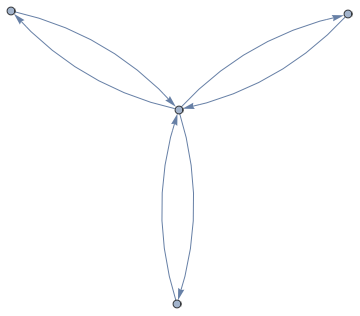
\includegraphics[width=0.5\linewidth]{img/star.png}
    \caption[Grafo estrella]{Grafo estrella}
    \label{fig:star}
\end{figure}

\begin{equation}
    A =
    \begin{pmatrix}
        0 & 1 & 1 & 1 \\
        1 & 0 & 0 & 0 \\
        1 & 0 & 0 & 0 \\
        1 & 0 & 0 & 0
    \end{pmatrix}
\end{equation}

\begin{equation}
    E = 
    \begin{pmatrix}
        0 & 1 & 1 & 1 \\
        \frac{1}{3} & 0 & 0 & 0 \\
        \frac{1}{3} & 0 & 0 & 0 \\
        \frac{1}{3} & 0 & 0 & 0
    \end{pmatrix}
\end{equation}

\begin{equation}
    G =
    \begin{pmatrix}
        \frac{3}{80} & \frac{71}{80} & \frac{71}{80} & \frac{71}{80} \\
        \frac{77}{240} & \frac{3}{80} & \frac{3}{80} & \frac{3}{80} \\
        \frac{77}{240} & \frac{3}{80} & \frac{3}{80} & \frac{3}{80} \\
        \frac{77}{240} & \frac{3}{80} & \frac{3}{80} & \frac{3}{80}
    \end{pmatrix}
\end{equation}

Los tres nodos exteriores de este grafo, además, forman lo que hemos llamado un subgrafo cíclico, por lo que para este grafo necesitaremos dos operadores $K_b$, unos para estos tres nodos y otro para el nodo central. Las figuras \ref{fig:starkb1} - \ref{fig:lokestar} muestran cómo construir el circuito del operador de difusión de la caminata de Szegedy asociada a la matriz de Google de este grafo.

\begin{figure}[H]
\[\Qcircuit @C=1.4em @R=1.8em {
& \gate{Ry(1.85806)} & \ctrlo{1}           & \ctrl{1}          & \qw \\
& \qw                & \gate{Ry(2.48274)}  & \gate{Ry(1.5708)} & \qw \\
} \]
\caption{Circuito de $K_1$ para el grafo estrella}
\label{fig:starkb1}
\end{figure}

\begin{figure}[H]
\[\Qcircuit @C=1.4em @R=1.8em {
& \gate{Ry(0.554811)} & \ctrlo{1}            & \ctrl{1}          & \qw \\
& \qw                 & \gate{Ry(0.405465)}  & \gate{Ry(1.5708)} & \qw \\
} \]
\caption{Circuito de $K_2$ para el grafo estrella}
\label{fig:starkb2}
\end{figure}

\begin{figure}[H]
\[\Qcircuit @C=1.4em @R=1.8em {
& \ctrlo{1}                   & \qw                 & \ctrlo{1}           & \qw \\
& \ctrlo{1}                   & \qw                 & \ctrlo{1}           & \qw \\
& \multigate{1}{K_1^\dagger} & \multigate{1}{K_1} & \multigate{1}{K_2} & \qw \\
& \ghost{K_1^\dagger}        & \ghost{K_1}        & \ghost{K_2}        & \qw \\
} 
\]
\caption[$K_b$ del grafo estrella]{$K_b$ del grafo estrella}
\label{fig:starkb}
\end{figure}

\begin{figure}[H]
\[\Qcircuit @C=1.4em @R=1.8em {
& \gate{Id} & \qw \\
& \gate{Id} & \qw \\
} 
\]
\caption[$T$ del grafo estrella]{$T$ del grafo estrella}
\label{fig:starT}
\end{figure}

\begin{figure}[H]
\[\Qcircuit @C=1.4em @R=1.8em {
& \gate{H} & \multigate{3}{K_b} & \qw \\
& \gate{H} & \ghost{K_b}        & \qw \\
& \qw      & \ghost{K_b}        & \qw \\
& \qw      & \ghost{K_b}        & \qw \\
} 
\]
\caption{Preparación del estado inicial para la caminata en el grafo estrella}
\label{fig:starinit}
\end{figure}

\begin{figure}[H]
\[ \Qcircuit @C=1.4em @R=1.8em {
\lstick{\ket{0}} & {/^4} \qw & \gate{Init} & \gate{K_b^\dagger} & \gate{D} & \gate{K_b} & \gate{SWAP} & \meter & \cw \\
                 & & & & \rstick{2m \text{ veces}}
\gategroup{1}{4}{1}{7}{1.3em}{_\}}
} \]
\caption{Circuito del PageRank cuántico  del grafo estrella}
\label{fig:lokestar}
\end{figure}

En la figura \ref{fig:inststarlossless} se puede observar la gráfica del PageRank cuántico instantáneo sin relajación. En esta figura se puede observar claramente la naturaleza sinusoidal de este algoritmo, por estar basado en reflexiones. Como se puede observar, ambas figuras son bastante similares. La diferencia está en que en el caso de la simulación matemática, el PageRank cuántico de los tres nodos exteriores se solapan perfectamente, mientras que en la simulación circuital, no. Esto se debe a la limitada precisión numérica del solucionador de ecuaciones maestras.

\begin{figure}[H]
    \centering
    \begin{subfigure}[m]{0.45\textwidth}
        \centering
        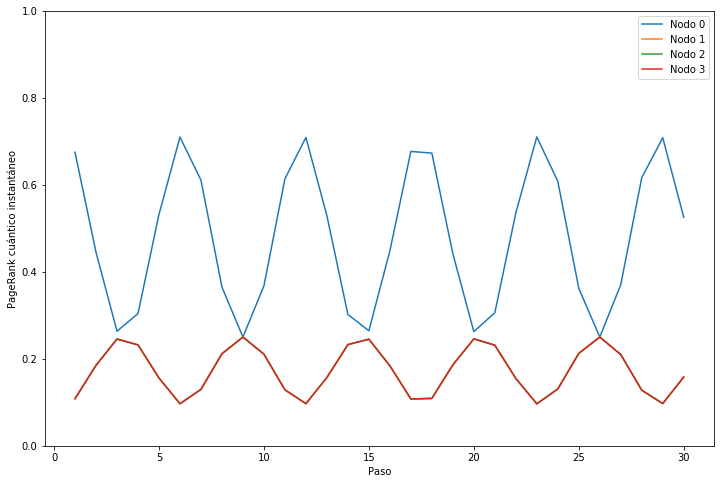
\includegraphics[width=0.9\linewidth]{img/star-inst-M.png}
        \caption{Wolfram Mathematica}
    \end{subfigure}
    \begin{subfigure}[m]{0.45\textwidth}
        \centering
        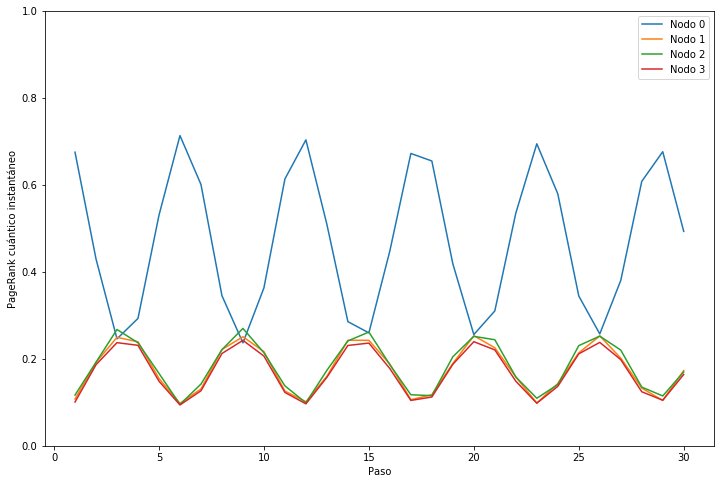
\includegraphics[width=0.9\linewidth]{img/star-inst-lossless.png}
        \caption{Python}
    \end{subfigure}
    \caption[PageRank cuántico instantáneo del grafo estrella sin pérdidas]{PageRank cuántico instantáneo del grafo estrella sin pérdidas}
    \label{fig:inststarlossless}
\end{figure}

En el caso del PageRank promedio, en la figura \ref{fig:meanstarlossless} podemos ver cómo este valor sí converge, a diferencia del PageRank instantaneo, el cuál oscila alrededor del valor de convergencia del PageRank promedio.

\begin{figure}[H]
    \centering
    \begin{subfigure}[m]{0.45\textwidth}
        \centering
        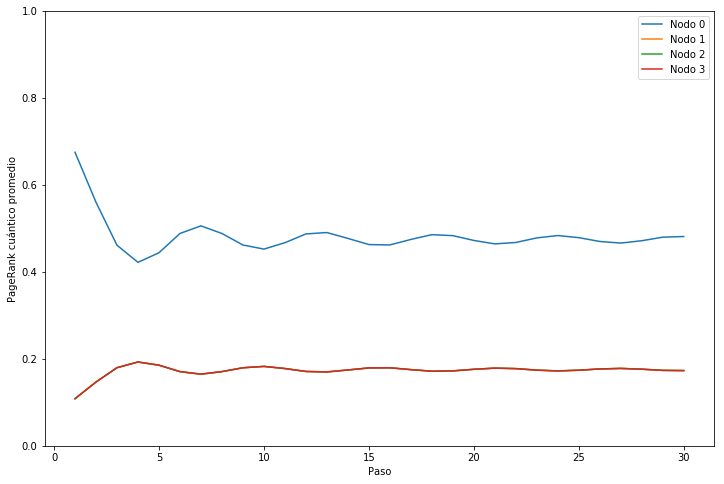
\includegraphics[width=0.9\linewidth]{img/star-mean-M.png}
        \caption{Wolfram Mathematica}
    \end{subfigure}
    \begin{subfigure}[m]{0.45\textwidth}
        \centering
        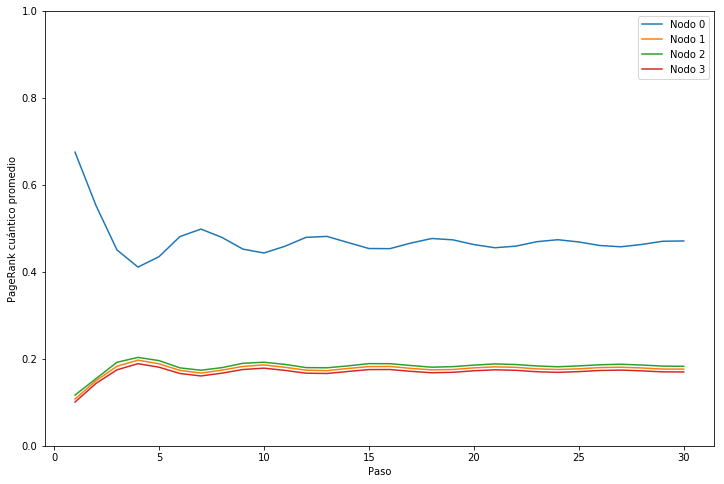
\includegraphics[width=0.9\linewidth]{img/star-mean-lossless.png}
        \caption{Python}
    \end{subfigure}
    \caption[PageRank cuántico promedio del grafo estrella sin pérdidas]{PageRank cuántico promedio del grafo estrella sin pérdidas}
    \label{fig:meanstarlossless}
\end{figure}

Ahora, compararemos los resultados de la simulación circuital con y sin pérdidas. Como se puede ver en la figura (FIGURA), en el caso con pérdidas, <++>

\begin{figure}[H]
    \centering
    \begin{subfigure}[m]{0.45\textwidth}
        \centering
        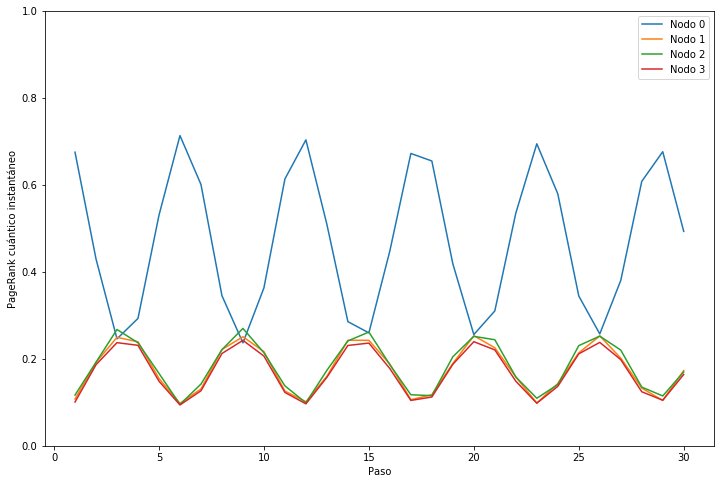
\includegraphics[width=0.9\linewidth]{img/star-inst-lossless.png}
        \caption{Sin relajación}
    \end{subfigure}
    \begin{subfigure}[m]{0.45\textwidth}
        \centering
        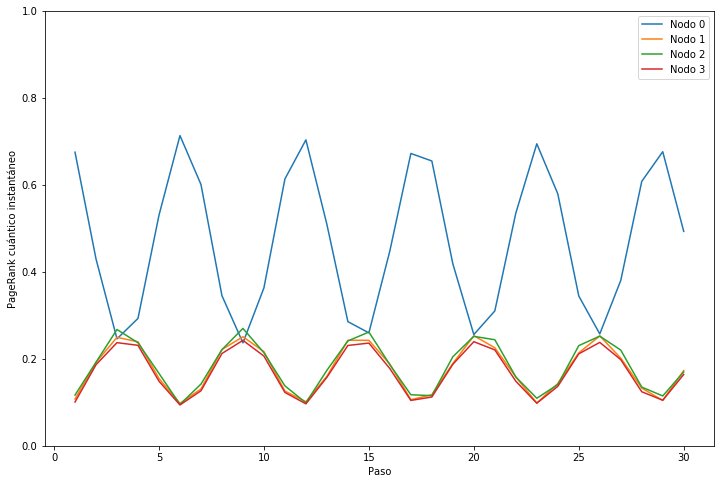
\includegraphics[width=0.9\linewidth]{img/star-inst-lossy.png}
        \caption{Con relajación}
    \end{subfigure}
    \caption[PageRank cuántico instantaneo del grafo estrella con y sin pérdidas]{PageRank cuántico instantaneo del grafo estrella con y sin pérdidas}
    \label{fig:inststarlossy}
\end{figure}

\begin{figure}[H]
    \centering
    \begin{subfigure}[m]{0.45\textwidth}
        \centering
        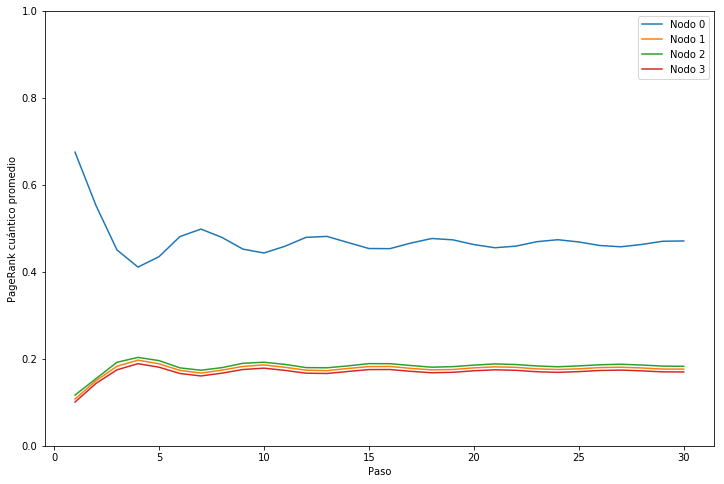
\includegraphics[width=0.9\linewidth]{img/star-mean-lossless.png}
        \caption{Sin relajación}
    \end{subfigure}
    \begin{subfigure}[m]{0.45\textwidth}
        \centering
        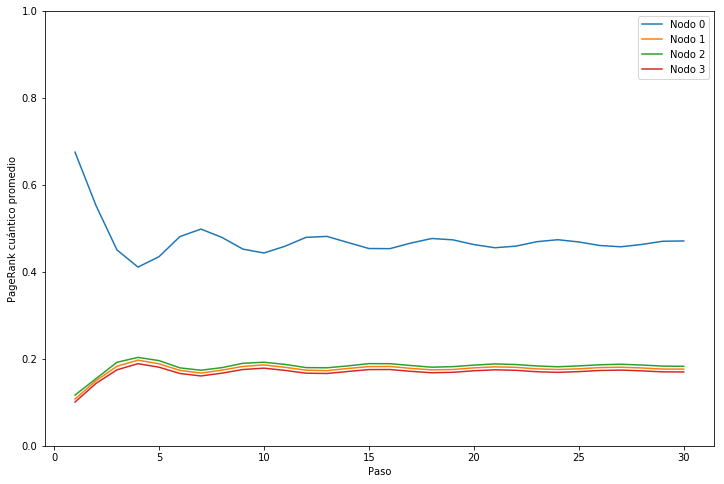
\includegraphics[width=0.9\linewidth]{img/star-mean-lossy.png}
        \caption{Con relajación}
    \end{subfigure}
    \caption[PageRank cuántico promedio del grafo estrella con y sin pérdidas]{PageRank cuántico promedio del grafo estrella con y sin pérdidas}
    \label{fig:meanstarlossy}
\end{figure}

\subsection{Grafo corona}

\begin{equation}
    A =
    \begin{pmatrix}
        0 & 1 & 1 & 0 \\
        1 & 0 & 1 & 0 \\
        1 & 1 & 0 & 0 \\
        1 & 1 & 1 & 0 \\
    \end{pmatrix}
\end{equation}

\begin{equation}
    E =
    \begin{pmatrix}
        0 & \frac{1}{3} & \frac{1}{3} & \frac{1}{4} \\
        \frac{1}{3} & 0 & \frac{1}{3} & \frac{1}{4} \\
        \frac{1}{3} & \frac{1}{3} & 0 & \frac{1}{4} \\
        \frac{1}{3} & \frac{1}{3} & \frac{1}{3} & \frac{1}{4} \\
    \end{pmatrix}
\end{equation}

\begin{equation}
    G =
    \begin{pmatrix}
        \frac{3}{80} & \frac{77}{240} & \frac{77}{240} & \frac{1}{4} \\
        \frac{77}{240} & \frac{3}{80} & \frac{77}{240} & \frac{1}{4} \\
        \frac{77}{240} & \frac{77}{240} & \frac{3}{80} & \frac{1}{4} \\
        \frac{77}{240} & \frac{77}{240} & \frac{77}{240} & \frac{1}{4} \\
    \end{pmatrix}
\end{equation}

\begin{figure}[H]
    \centering
    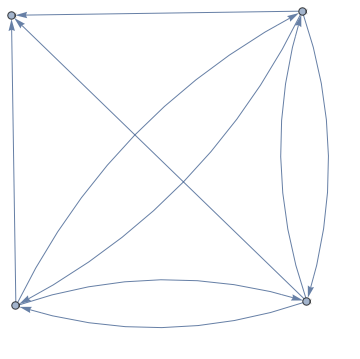
\includegraphics[width=0.5\linewidth]{img/crown.png}
    \caption[Grafo corona]{Grafo corona}
    \label{fig:crown}
\end{figure}

\begin{figure}[H]
    \centering
    \begin{subfigure}[m]{0.45\textwidth}
        \centering
        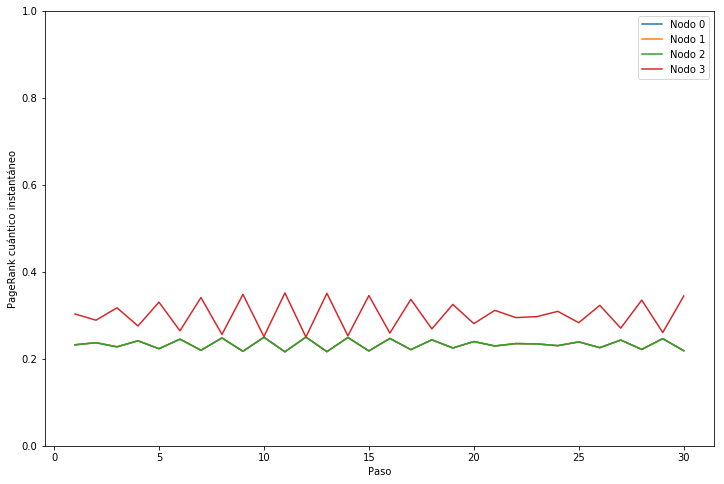
\includegraphics[width=0.9\linewidth]{img/crown-inst-M.png}
        \caption{Wolfram Mathematica}
    \end{subfigure}
    \begin{subfigure}[m]{0.45\textwidth}
        \centering
        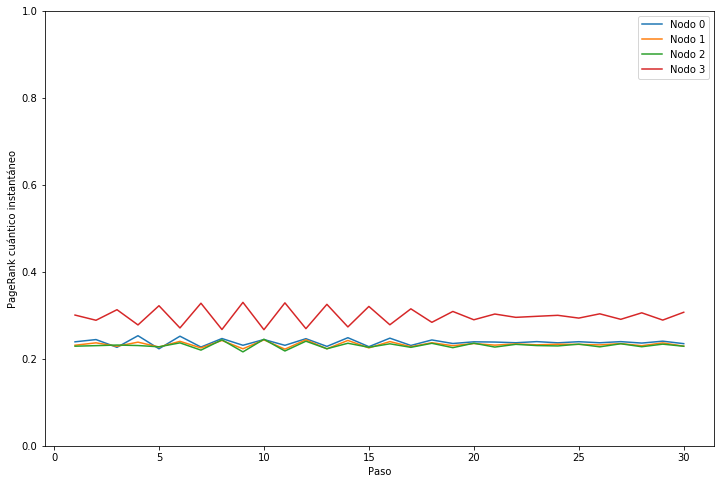
\includegraphics[width=0.9\linewidth]{img/crown-inst-lossless.png}
        \caption{Python}
    \end{subfigure}
    \caption[PageRank cuántico instantáneo del grafo corona sin pérdidas]{PageRank cuántico instantáneo del grafo corona sin pérdidas}
    \label{fig:instcrownlossless}
\end{figure}

\begin{figure}[H]
    \centering
    \begin{subfigure}[m]{0.45\textwidth}
        \centering
        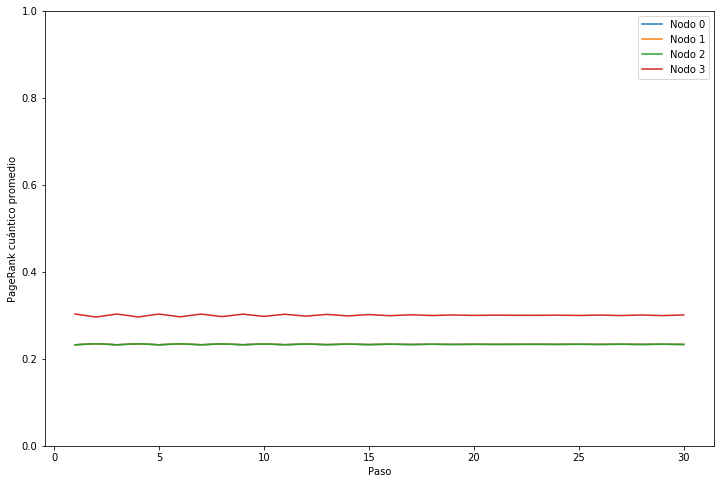
\includegraphics[width=0.9\linewidth]{img/crown-mean-M.png}
        \caption{Wolfram Mathematica}
    \end{subfigure}
    \begin{subfigure}[m]{0.45\textwidth}
        \centering
        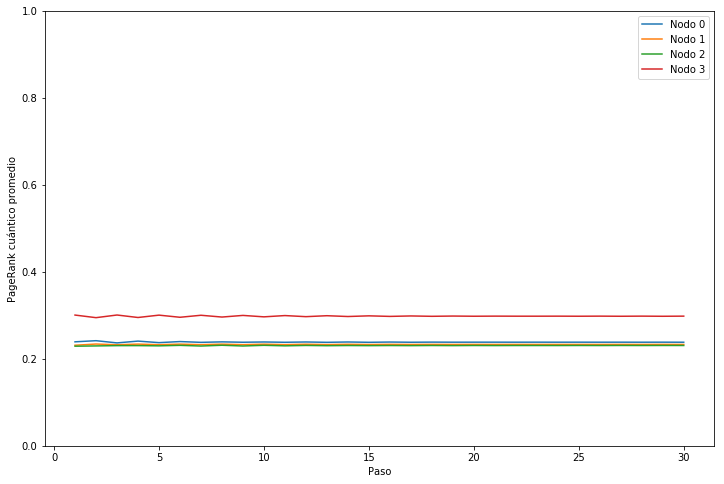
\includegraphics[width=0.9\linewidth]{img/crown-mean-lossless.png}
        \caption{Python}
    \end{subfigure}
    \caption[PageRank cuántico promedio del grafo corona sin pérdidas]{PageRank cuántico promedio del grafo corona sin pérdidas}
    \label{fig:meancrownlossless}
\end{figure}

\subsection{Grafo árbol}

\begin{equation}
    A = 
    \begin{pmatrix}
        0 & 0 & 0 & 0 \\
        1 & 0 & 0 & 0 \\
        1 & 0 & 0 & 0 \\
        0 & 1 & 0 & 0 \\
    \end{pmatrix}
\end{equation}

\begin{equation}
    E =
    \begin{pmatrix}
        0 & 0 & \frac{1}{4} & \frac{1}{4} \\
        \frac{1}{2} & 0 & \frac{1}{4} & \frac{1}{4} \\
        \frac{1}{2} & 0 & \frac{1}{4} & \frac{1}{4} \\
        0 & 1 & \frac{1}{4} & \frac{1}{4} \\
    \end{pmatrix}
\end{equation}

\begin{equation}
    G =
    \begin{pmatrix}
        \frac{3}{80} & \frac{3}{80} & \frac{1}{4} & \frac{1}{4} \\
        \frac{37}{80} & \frac{3}{80} & \frac{1}{4} & \frac{1}{4} \\
        \frac{37}{80} & \frac{3}{80} & \frac{1}{4} & \frac{1}{4} \\
        \frac{3}{80} & \frac{71}{80} & \frac{1}{4} & \frac{1}{4} \\
    \end{pmatrix}
\end{equation}

\begin{figure}[H]
    \centering
    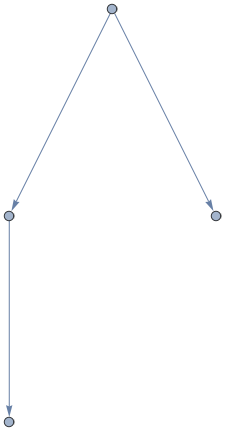
\includegraphics[width=0.5\linewidth]{img/tree.png}
    \caption[Grafo árbol]{Grafo árbol}
    \label{fig:tree}
\end{figure}

\begin{figure}[H]
    \centering
    \begin{subfigure}[m]{0.45\textwidth}
        \centering
        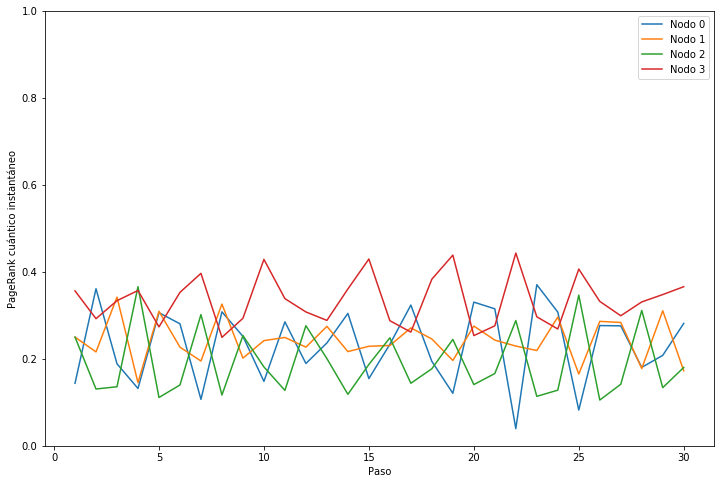
\includegraphics[width=0.9\linewidth]{img/tree-inst-M.png}
        \caption{Wolfram Mathematica}
    \end{subfigure}
    \begin{subfigure}[m]{0.45\textwidth}
        \centering
        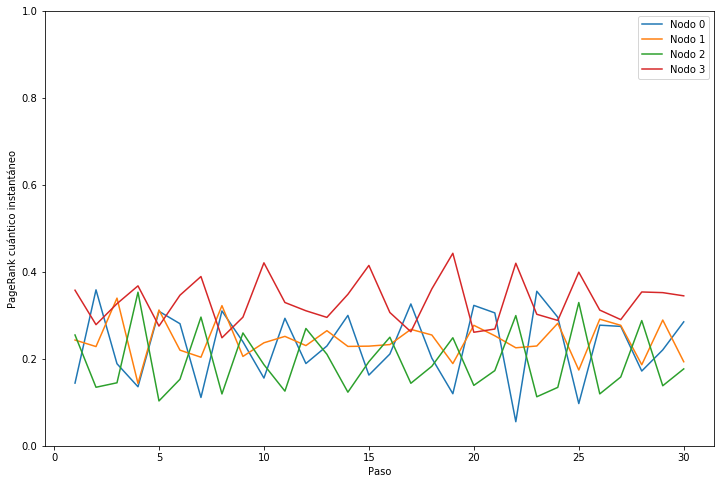
\includegraphics[width=0.9\linewidth]{img/tree-inst-lossless.png}
        \caption{Python}
    \end{subfigure}
    \caption[PageRank cuántico instantáneo del grafo árbol sin pérdidas]{PageRank cuántico instantáneo del grafo árbol sin pérdidas}
    \label{fig:insttreelossless}
\end{figure}

\begin{figure}[H]
    \centering
    \begin{subfigure}[m]{0.45\textwidth}
        \centering
        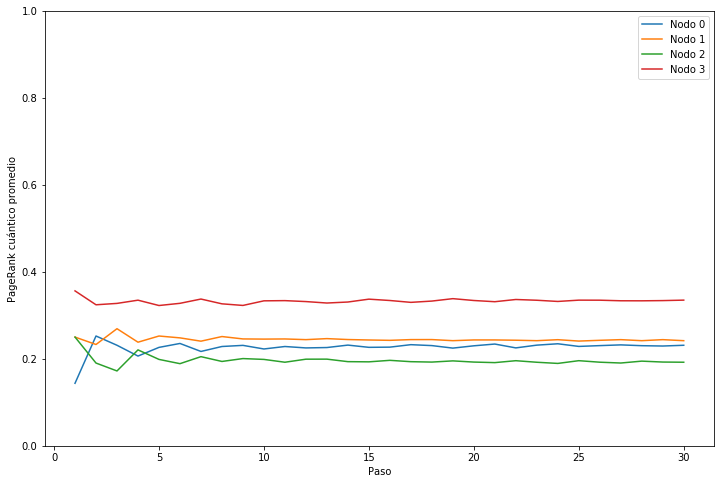
\includegraphics[width=0.9\linewidth]{img/tree-mean-M.png}
        \caption{Wolfram Mathematica}
    \end{subfigure}
    \begin{subfigure}[m]{0.45\textwidth}
        \centering
        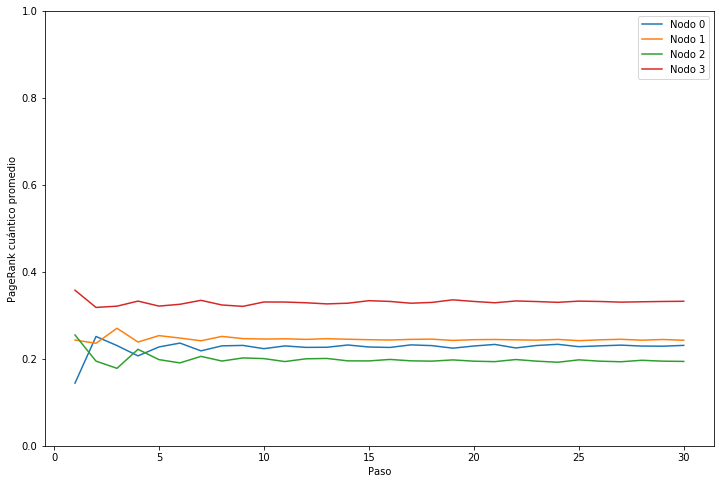
\includegraphics[width=0.9\linewidth]{img/tree-mean-lossless.png}
        \caption{Python}
    \end{subfigure}
    \caption[PageRank cuántico promedio del grafo árbol sin pérdidas]{PageRank cuántico promedio del grafo árbol sin pérdidas}
    \label{fig:meantreelossless}
\end{figure}

\begin{figure}[H]
    \centering
    \begin{subfigure}[m]{0.45\textwidth}
        \centering
        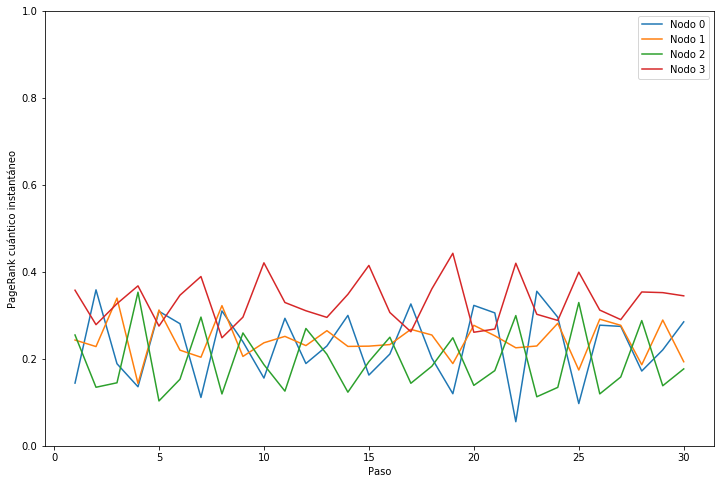
\includegraphics[width=0.9\linewidth]{img/tree-inst-lossless.png}
        \caption{Sin relajación}
    \end{subfigure}
    \begin{subfigure}[m]{0.45\textwidth}
        \centering
        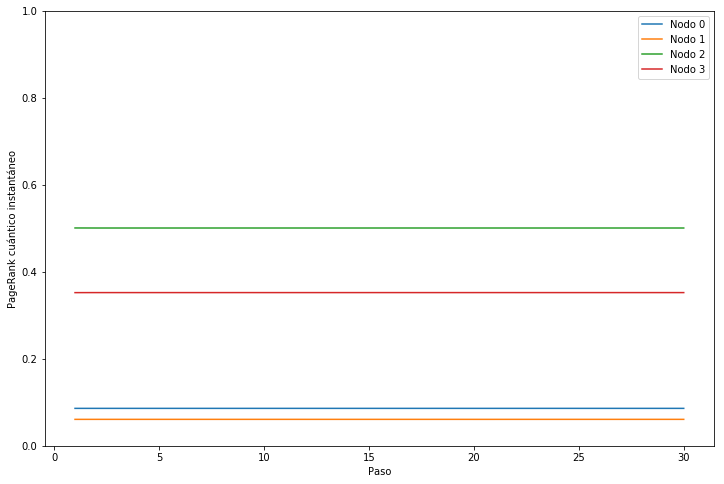
\includegraphics[width=0.9\linewidth]{img/tree-inst-lossy.png}
        \caption{Con relajación}
    \end{subfigure}
    \caption[PageRank cuántico instantaneo del grafo árbol con y sin pérdidas]{PageRank cuántico instantaneo del grafo árbol con y sin pérdidas}
    \label{fig:insttreelossy}
\end{figure}

\begin{figure}[H]
    \centering
    \begin{subfigure}[m]{0.45\textwidth}
        \centering
        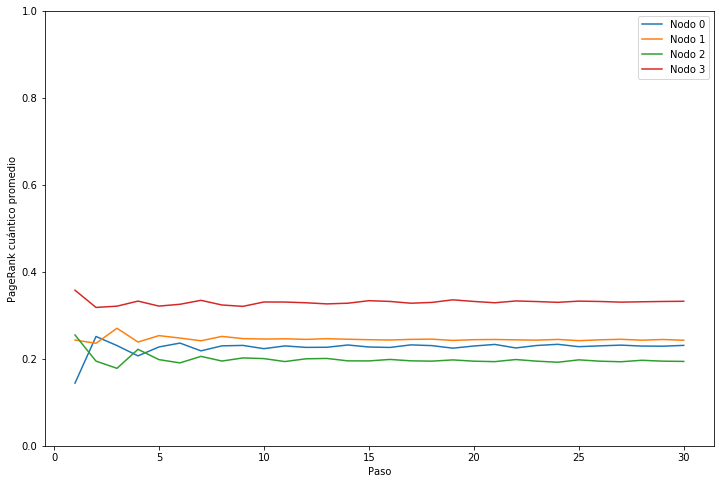
\includegraphics[width=0.9\linewidth]{img/tree-mean-lossless.png}
        \caption{Sin relajación}
    \end{subfigure}
    \begin{subfigure}[m]{0.45\textwidth}
        \centering
        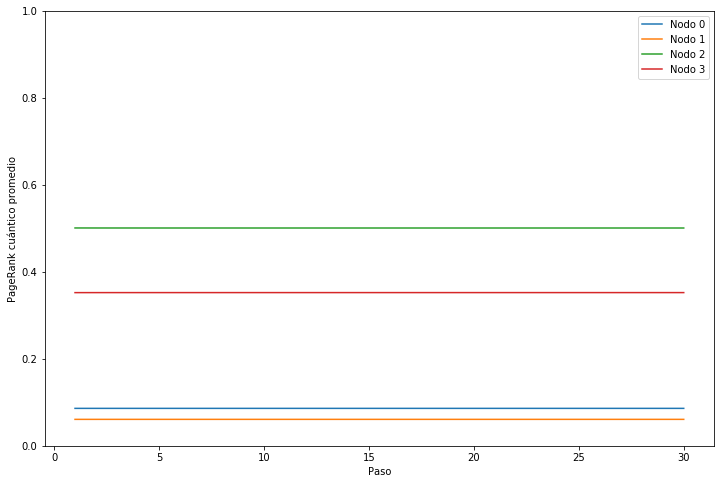
\includegraphics[width=0.9\linewidth]{img/tree-mean-lossy.png}
        \caption{Con relajación}
    \end{subfigure}
    \caption[PageRank cuántico promedio del grafo árbol con y sin pérdidas]{PageRank cuántico promedio del grafo árbol con y sin pérdidas}
    \label{fig:meantreelossy}
\end{figure}

\subsection{Grafo aleatorio}

\begin{equation}
    A =
    \begin{pmatrix}
        0 & 1 & 0 & 0 \\
        1 & 0 & 0 & 0 \\
        1 & 0 & 0 & 1 \\
        1 & 1 & 1 & 0 \\
    \end{pmatrix}
\end{equation}

\begin{equation}
    E =
    \begin{pmatrix}
        0 & \frac{1}{2} & 0 & 0 \\
        \frac{1}{3} & 0 & 0 & 0 \\
        \frac{1}{3} & 0 & 0 & 1 \\
        \frac{1}{3} & \frac{1}{2} & 1 & 0 \\
    \end{pmatrix}
\end{equation}

\begin{equation}
    G =
    \begin{pmatrix}
        \frac{3}{80} & \frac{37}{80} & \frac{3}{80} & \frac{3}{80} \\
        \frac{77}{240} & \frac{3}{80} & \frac{3}{80} & \frac{3}{80} \\
        \frac{77}{240} & \frac{3}{80} & \frac{3}{80} & \frac{71}{80} \\
        \frac{77}{240} & \frac{37}{80} & \frac{71}{80} & \frac{3}{80} \\
    \end{pmatrix}
\end{equation}

\begin{figure}[H]
    \centering
    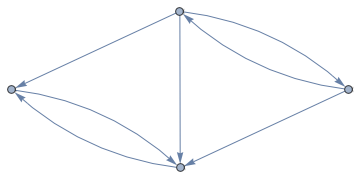
\includegraphics[width=0.5\linewidth]{img/any.png}
    \caption[Grafo aleatorio]{Grafo aleatorio}
    \label{fig:any}
\end{figure}

\begin{figure}[H]
    \centering
    \begin{subfigure}[m]{0.45\textwidth}
        \centering
        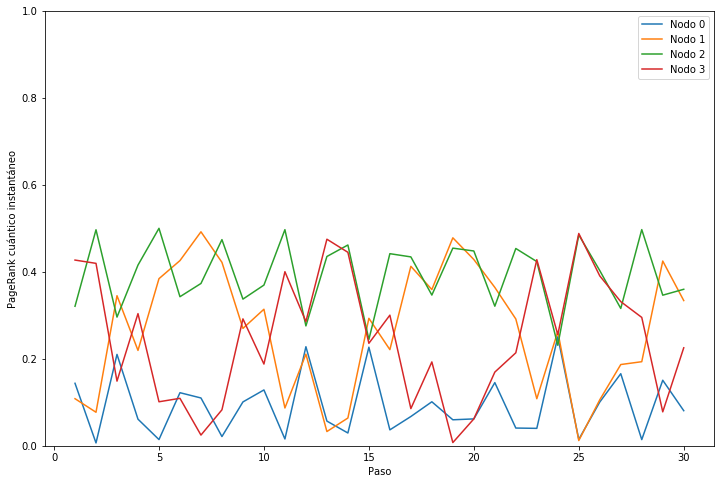
\includegraphics[width=0.9\linewidth]{img/any-inst-M.png}
        \caption{Wolfram Mathematica}
    \end{subfigure}
    \begin{subfigure}[m]{0.45\textwidth}
        \centering
        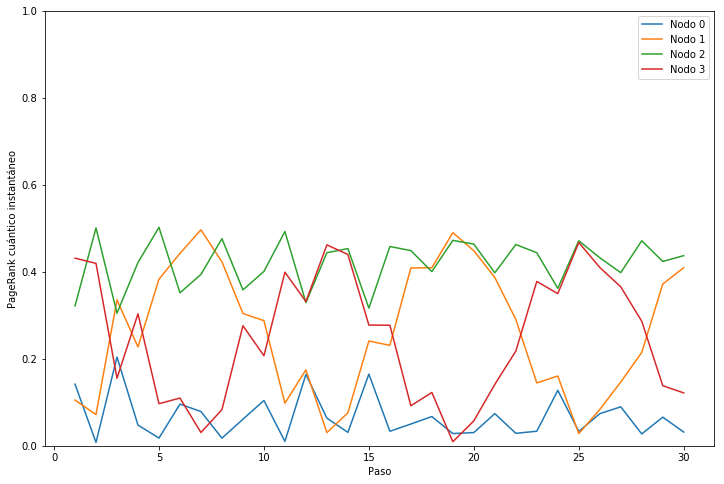
\includegraphics[width=0.9\linewidth]{img/any-inst-lossless.png}
        \caption{Python}
    \end{subfigure}
    \caption[PageRank cuántico instantáneo del grafo aleatorio sin pérdidas]{PageRank cuántico instantáneo del grafo aleatorio sin pérdidas}
    \label{fig:instanylossless}
\end{figure}

\begin{figure}[H]
    \centering
    \begin{subfigure}[m]{0.45\textwidth}
        \centering
        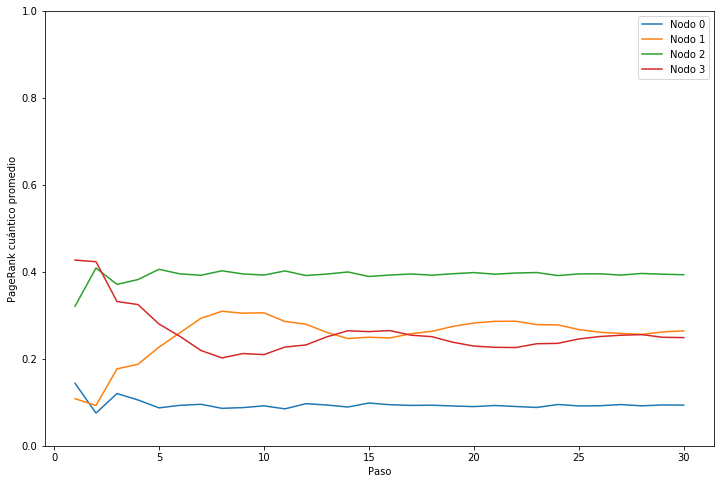
\includegraphics[width=0.9\linewidth]{img/any-mean-M.png}
        \caption{Wolfram Mathematica}
    \end{subfigure}
    \begin{subfigure}[m]{0.45\textwidth}
        \centering
        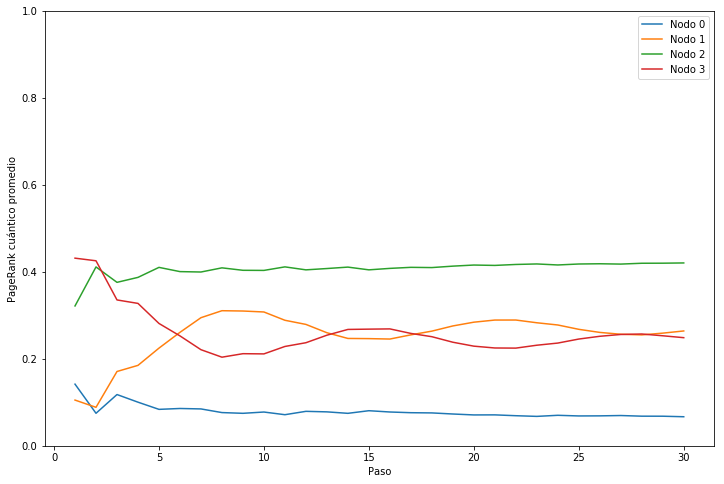
\includegraphics[width=0.9\linewidth]{img/any-mean-lossless.png}
        \caption{Python}
    \end{subfigure}
    \caption[PageRank cuántico promedio del grafo aleatorio sin pérdidas]{PageRank cuántico promedio del grafo aleatorio sin pérdidas}
    \label{fig:meananylossless}
\end{figure}

\begin{figure}[H]
    \centering
    \begin{subfigure}[m]{0.45\textwidth}
        \centering
        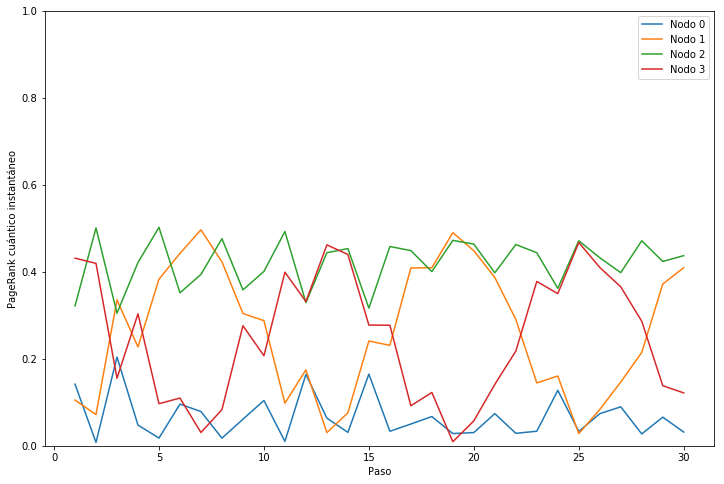
\includegraphics[width=0.9\linewidth]{img/any-inst-lossless.png}
        \caption{Sin relajación}
    \end{subfigure}
    \begin{subfigure}[m]{0.45\textwidth}
        \centering
        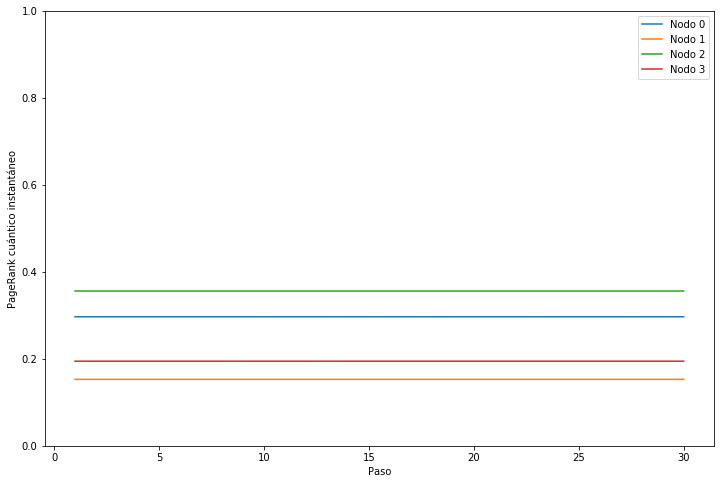
\includegraphics[width=0.9\linewidth]{img/any-inst-lossy.png}
        \caption{Con relajación}
    \end{subfigure}
    \caption[PageRank cuántico instantaneo del grafo aleatorio con y sin pérdidas]{PageRank cuántico instantaneo del grafo aleatorio con y sin pérdidas}
    \label{fig:instanylossy}
\end{figure}

\begin{figure}[H]
    \centering
    \begin{subfigure}[m]{0.45\textwidth}
        \centering
        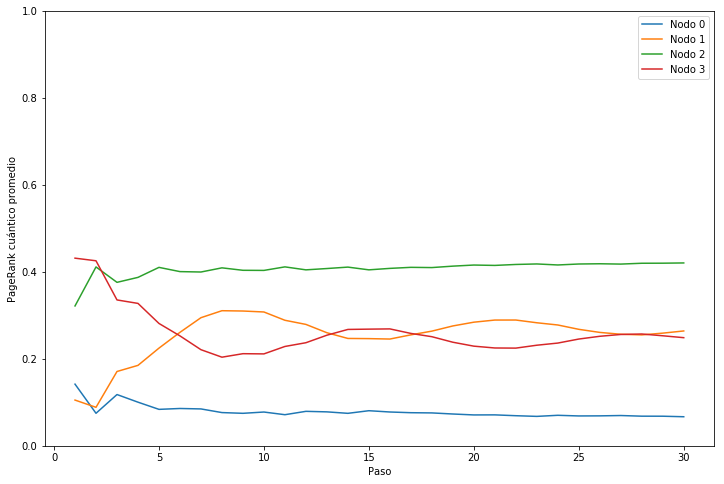
\includegraphics[width=0.9\linewidth]{img/any-mean-lossless.png}
        \caption{Sin relajación}
    \end{subfigure}
    \begin{subfigure}[m]{0.45\textwidth}
        \centering
        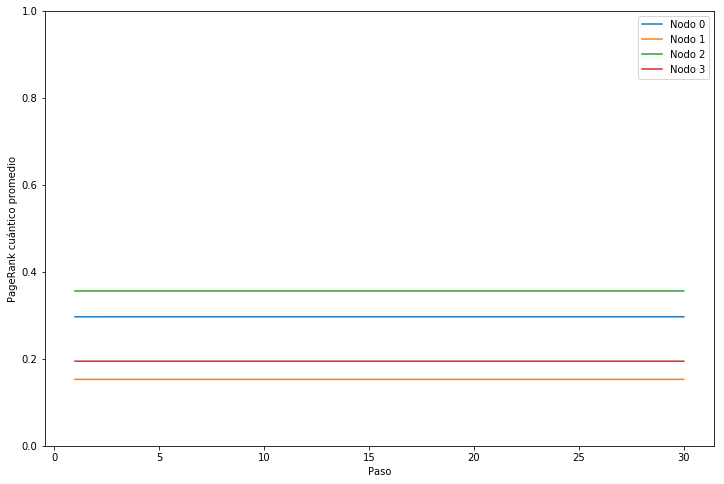
\includegraphics[width=0.9\linewidth]{img/any-mean-lossy.png}
        \caption{Con relajación}
    \end{subfigure}
    \caption[PageRank cuántico promedio del grafo aleatorio con y sin pérdidas]{PageRank cuántico promedio del grafo aleatorio con y sin pérdidas}
    \label{fig:meananylossy}
\end{figure}



